Il existe une relation entre le Marché de Gros et le (ou les) PONE. Cette relation est unidirectionnel en User Datagramme Packet ( UDP ), nous envoyons des datagrammes packets du Pone contenant une énergie qui est caractérisée par :
\\
\begin{itemize}
    \item Un type d'energie,
    \item Une quantité envoyé,
    \item Un mode d'extraction,
    \item Un prix unitaire,
    \item Un numéro de lot
    \\
\end{itemize}
 Cette énergie est donc envoyée vers les marché de gros sans vérification d'aquisition car l'UDP est un protocole de transite d'informations sur internet qui n'est pas en capacité de garantir la bonne récéption des informations chez le client.
\begin{figure}[h]
    \centering
    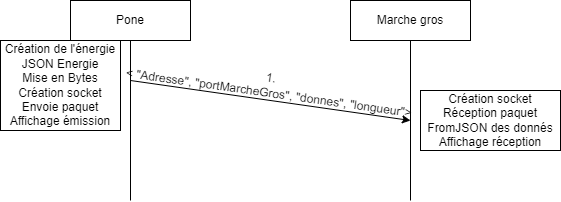
\includegraphics[width=120mm, height=45mm]{images/PONEMG.png}
    \caption{Modélisation de la relation entre Marché de Gros et PONE}
    \label{img:mesh16}
\end{figure}
